\documentclass[compress]{beamer}
\usepackage{ifthen}

\title{CMS Program Part II: \\ Muon Chambers and Muon-Related Analyses}
\author{Jim Pivarski}
\institute{Texas A\&M University}
\date{22 January, 2007}

\setbeamertemplate{navigation symbols}{}
\setbeamertemplate{headline}{\includegraphics[height=1 cm]{../cmslogo} \hspace{0.1 cm} \includegraphics[height=1 cm]{../tamulogo} \hfill
\begin{minipage}{9 cm}
\vspace{-0.75 cm} \small
\begin{center}
\ifthenelse{\equal{\insertpagenumber}{1}}{}{\insertsection}
\end{center}
\end{minipage} \hfill
\begin{minipage}{1 cm}
\vspace{-0.75 cm} \small
\begin{center}
\ifthenelse{\equal{\insertpagenumber}{1}}{}{\insertpagenumber/\pageref{numpages}}
\end{center}
\end{minipage}}

%\xdefinecolor{verylightgray}{rgb}{0.95,0.95,0.95}
%\beamertemplateshadingbackground{verylightgray}{white}

\begin{document}
\frame{\titlepage}

\begin{frame}
\frametitle{Organization of this talk}
\begin{itemize}\setlength{\itemsep}{0.5 cm}
  \item Muon Experience from CDF
  \item CMS EMU Projects: Low Voltage and Alignment
  \item $Z'\to\mu\mu$ Search
  \item Aligning Muon Chambers with Tracks (software)
  \item Hardware EMU Alignment
  \item Super-LHC Upgrade
\end{itemize}
\end{frame}

\section*{Muons at CDF --- Jim Pivarski}

\begin{frame}
\frametitle{A\&M's muon experience at CDF}

\begin{minipage}{0.8\linewidth}
  \begin{itemize}\setlength{\itemsep}{1 cm}
    \item Muon Reconstruction (Kamon, Krutelyov)

    \vspace{0.25 cm}
    \begin{itemize}\setlength{\itemsep}{0.25 cm}
      \item SimpleExtrapolator matches central tracker tracks to muon stubs
      \item Fast and accurate
      \item Now part of standard CDF muon reconstruction
    \end{itemize}

    \item Low $p_T$ di-muon trigger (Kamon, Krutelyov)

    \vspace{0.25 cm}
    \begin{itemize}
      \item Used to search for $B_s\to\mu\mu$
    \end{itemize}

  \end{itemize}
\end{minipage}
\end{frame}

\begin{frame}
\frametitle{SUSY constraint through $B_s \to \mu\mu$}
\begin{tabular}{p{0.68\linewidth} p{0.4\linewidth}}
  \hspace{-1 cm}
  \begin{minipage}{\linewidth}
    \begin{itemize}\setlength{\itemsep}{0.4 cm}
      \item Co-proposed by Kamon, previously overlooked test of SUSY
      \item One of the strongest CDF constraints on high $\tan\beta$ SUSY
      \item World's best upper limit $\mathcal{B} < 1.0\times 10^{-7}$ \\ at 95\% C.L.\ (780 pb$^{-1}$)
      \item First SUSY paper from CDF Run II
      \item We are using a neural net and extending to 1 fb$^{-1}$ (Weinberger, Kamon)
      \item Interested in continuing at CMS
    \end{itemize}
  \end{minipage} &
  \hspace{-1.3 cm}
  \begin{minipage}{\linewidth}
    \vspace{-1 cm}
    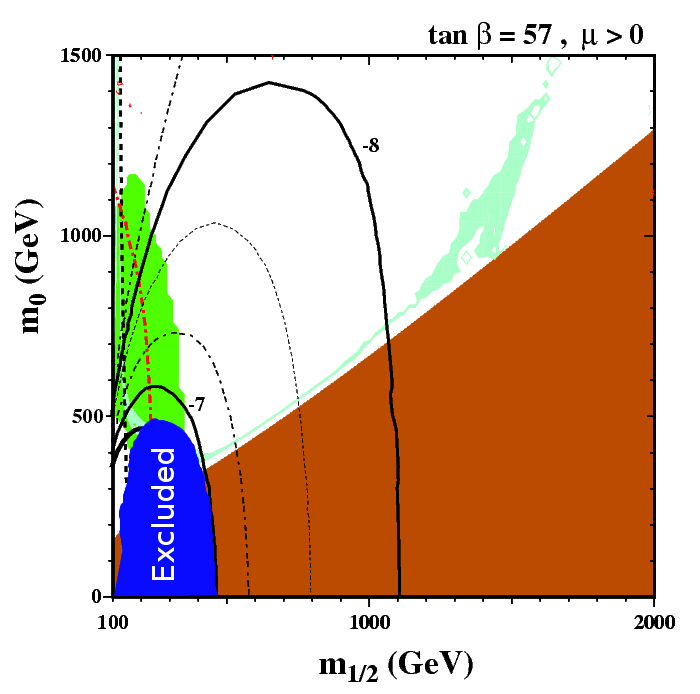
\includegraphics[width=\linewidth]{plots/bs_to_mumu/standard_susy_plane2}

    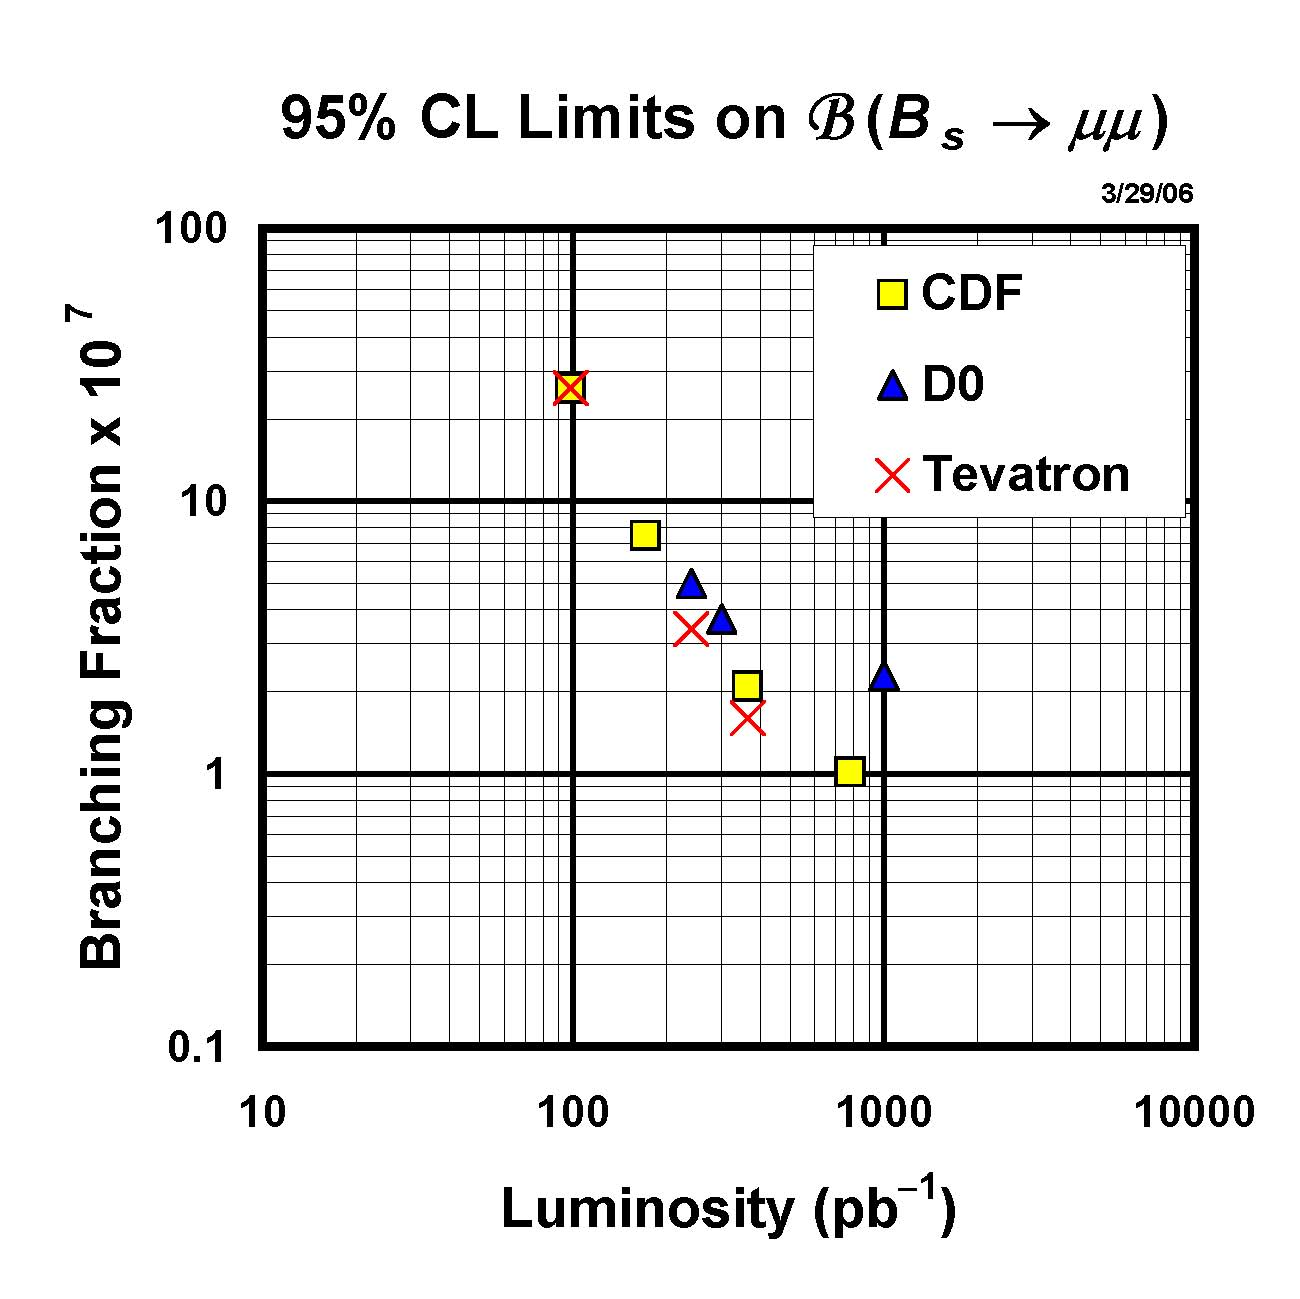
\includegraphics[width=\linewidth]{plots/Bs2mumu_95CL_060323}
  \end{minipage}
\end{tabular}
\end{frame}

\section*{Endcap Muon Chambers at CMS --- Jim Pivarski}

\begin{frame}
\frametitle{A\&M's involvement in CMS EMU}
\begin{itemize}\setlength{\itemsep}{0.25 cm}
  \item Good fit to our interests and experience
  \item EMU members since June 2006
  \item Took charge of critical areas:
  \begin{itemize}
    \item Low voltage power supply
    \item Chamber alignment
  \end{itemize}
    \vspace{-3.25 cm}
  \item<2> Hired Alexander Golyash July 2006 \hfill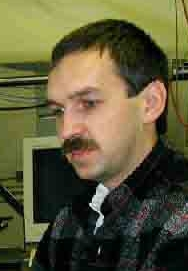
\includegraphics[width=2.5 cm]{plots/sasha2.png}
  \begin{itemize}
    \item lead engineer on construction and commissioning of low voltage
    \item will provide long-term support
  \end{itemize}
  \item<2> Hired Jim Pivarski (me) September 2006
  \begin{itemize}
    \item wrote muon alignment software
    \item developing an alignment strategy
    \item will study $Z' \to \mu\mu$
  \end{itemize}
\end{itemize}
\end{frame}

\begin{frame}
\frametitle{Low voltage power supply}
\vspace{-0.3 cm}
\begin{itemize}
  \item Powers trigger/read-out crates and on-board electronics
  \item Even though it's a part of a subsystem, it's an involved project
\end{itemize}

\vspace{0.3 cm}
\begin{tabular}{p{0.35\linewidth} p{0.6\linewidth}}
  \begin{minipage}{\linewidth}
    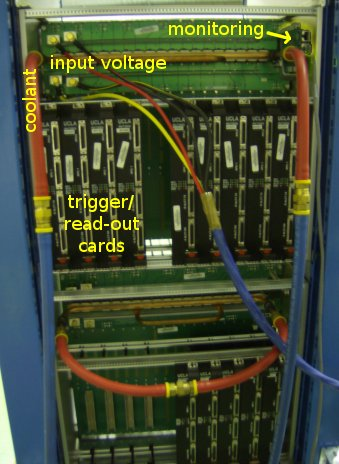
\includegraphics[width=\linewidth]{plots/teststand_back.jpg}
  \end{minipage} &
  \begin{minipage}{\linewidth}
    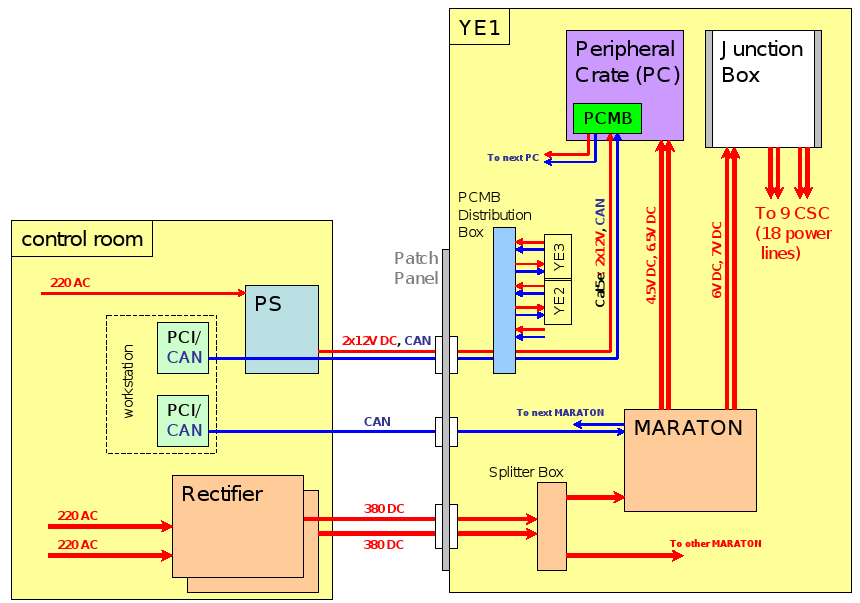
\includegraphics[width=\linewidth]{plots/lowvolt/low_voltage_system}
  \end{minipage}
\end{tabular}
\end{frame}

\begin{frame}
\frametitle{Monitoring low voltage}
\begin{tabular}{p{0.26\linewidth} p{0.7\linewidth}}
  \begin{minipage}{\linewidth}
    \vspace{0.5 cm} \hspace{-0.7 cm} 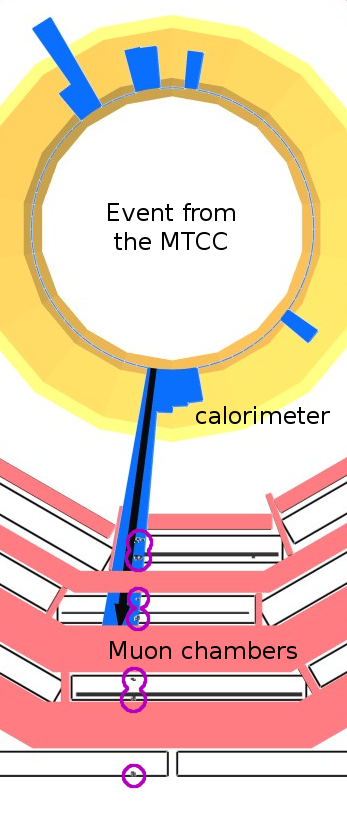
\includegraphics[width=\linewidth]{plots/Run2269_Ev61.png}
  \end{minipage} &
  \hspace{-1 cm}
  \begin{minipage}{1.2\linewidth}
    \begin{itemize}
      \item Recorded voltages and currents from MTCC (summer 2006 slice test)
      \item Needed a way to organize large logfiles
      \item We developed an expert tool for diagnostics
    \end{itemize}
    \begin{center}
      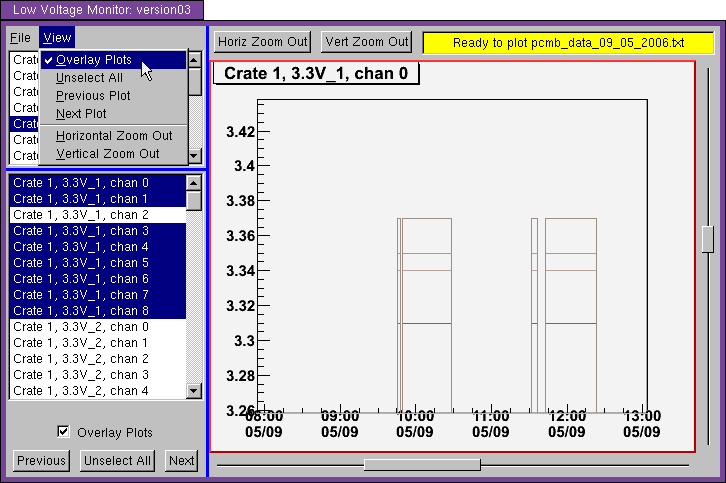
\includegraphics[width=0.67\linewidth]{plots/mine/lowvolt.png}
    \end{center}
  \end{minipage}
\end{tabular}
\end{frame}

\begin{frame}
\frametitle{There's still a lot of work to be done}
\begin{center}
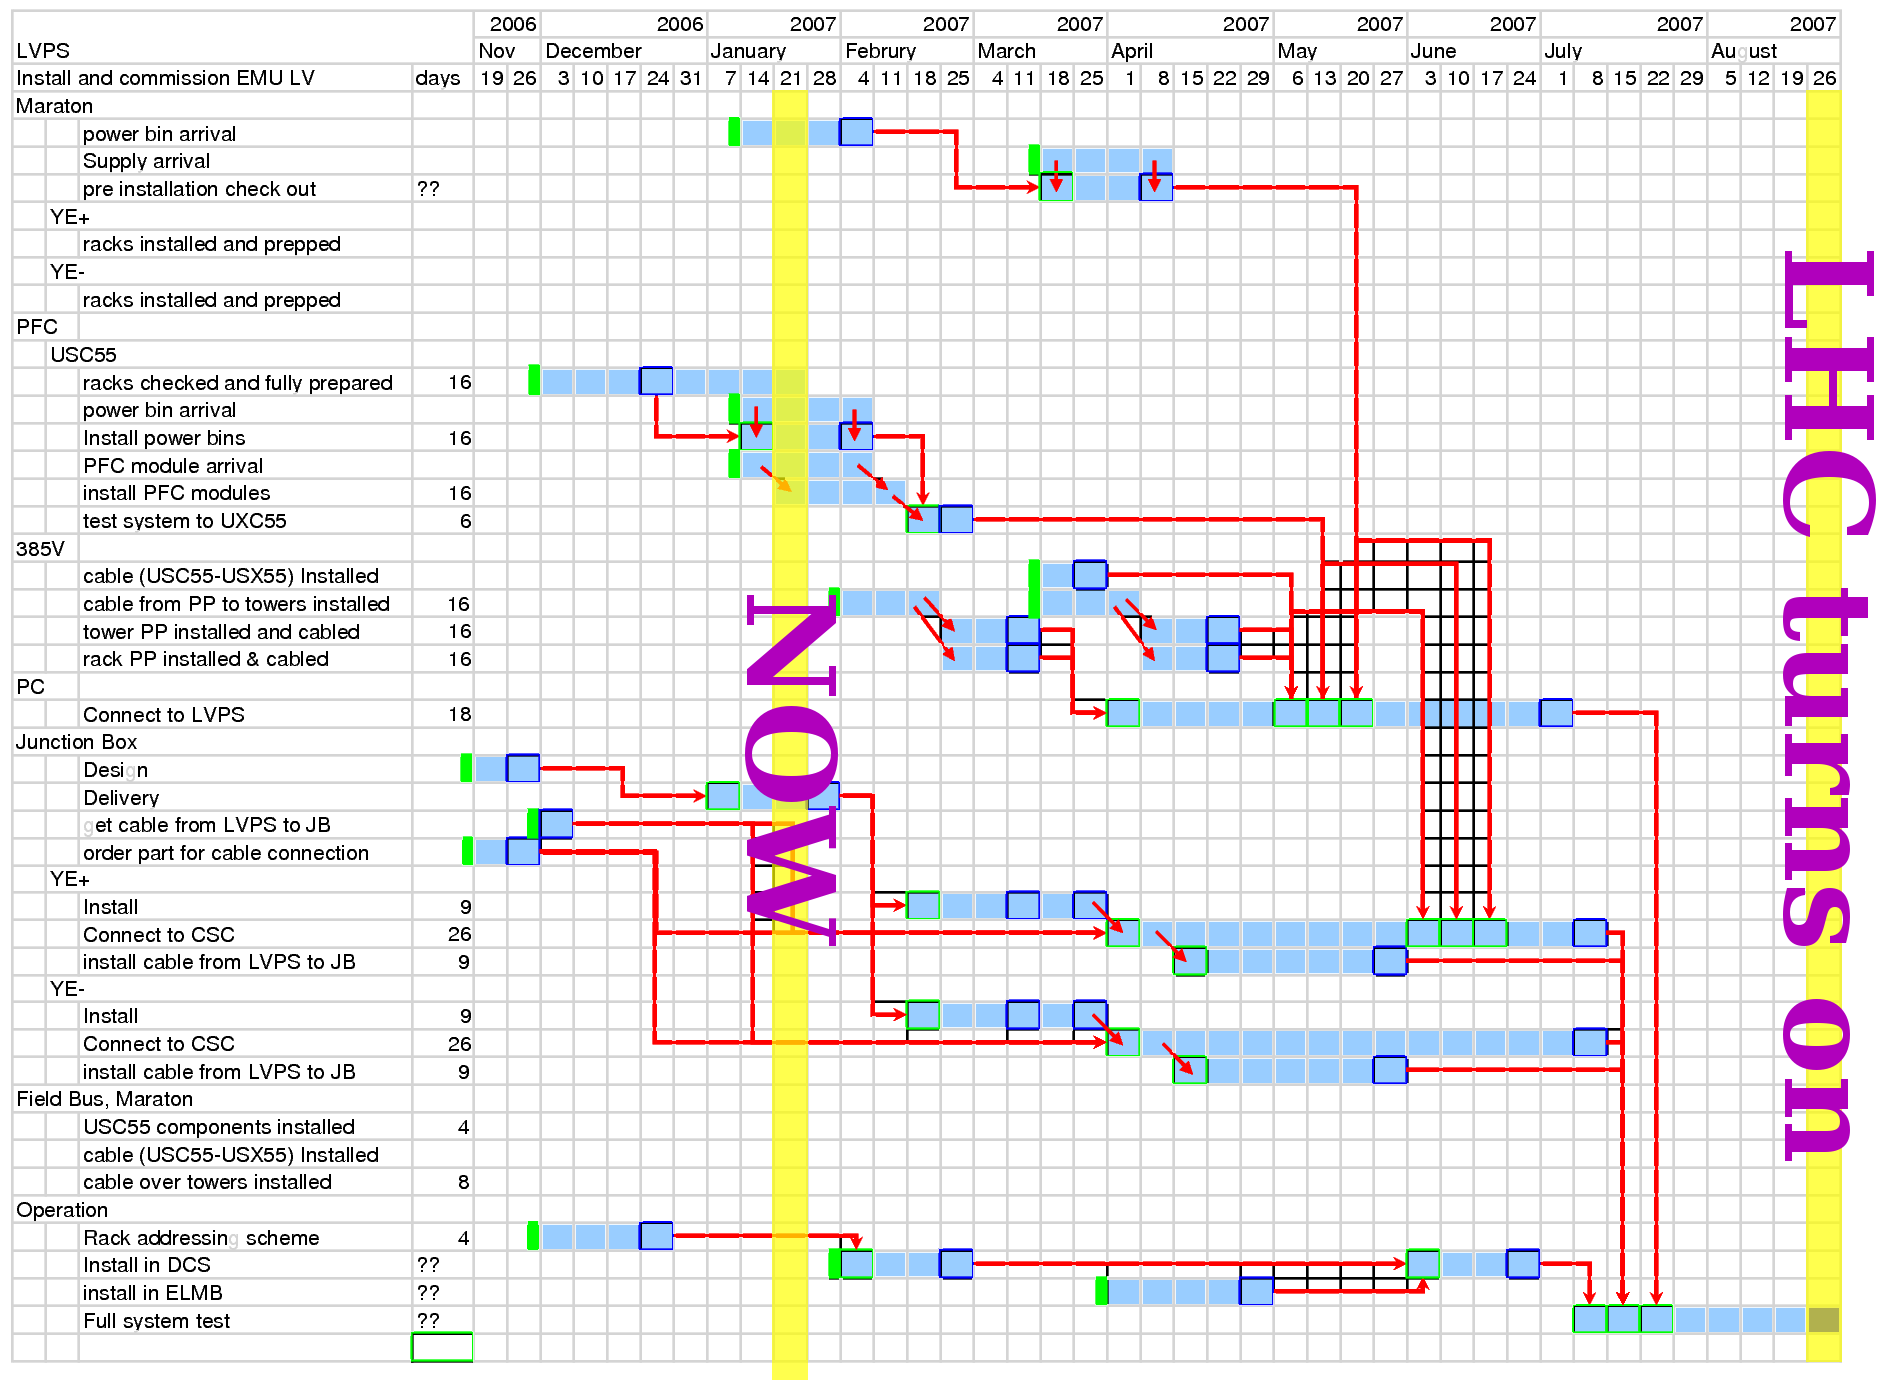
\includegraphics[width=0.6\linewidth]{plots/lowvolt/sashas_schedule.png}
\end{center}

\vspace{-0.5 cm}
\begin{itemize}
  \item Ordered components, shipping schedule is tight
  \item Need to coordinate with other projects for electricity, lifts,
  and space underground
\end{itemize}
\end{frame}

\section*{Interest in $Z'$ Search --- Jim Pivarski}

\begin{frame}
\frametitle{Physics interest: $Z'\to\mu\mu$}

Many theories predict a heavy neutral boson, generically called $Z'$

\begin{itemize}
  \item Unification gauge groups
  \item Excitation of $Z^0$ or graviton in extra dimensions
  \item $\tilde{\nu}$ in R-parity violating SUSY
\end{itemize}

\vfill Experimentally striking feature: \\
\hspace{1.5 cm} a peak in $\mu\mu$, $e^+e^-$, and di-jet mass spectra

\vfill (A concrete way to search for New Phyics model-independently!)

\vfill \bf Early CMS result!
\end{frame}

\begin{frame}
\frametitle{$Z'\to\mu\mu$ signal is diluted by misalignment}

\begin{tabular}{p{0.45\linewidth} p{0.45\linewidth}}
  \begin{minipage}{\linewidth}
    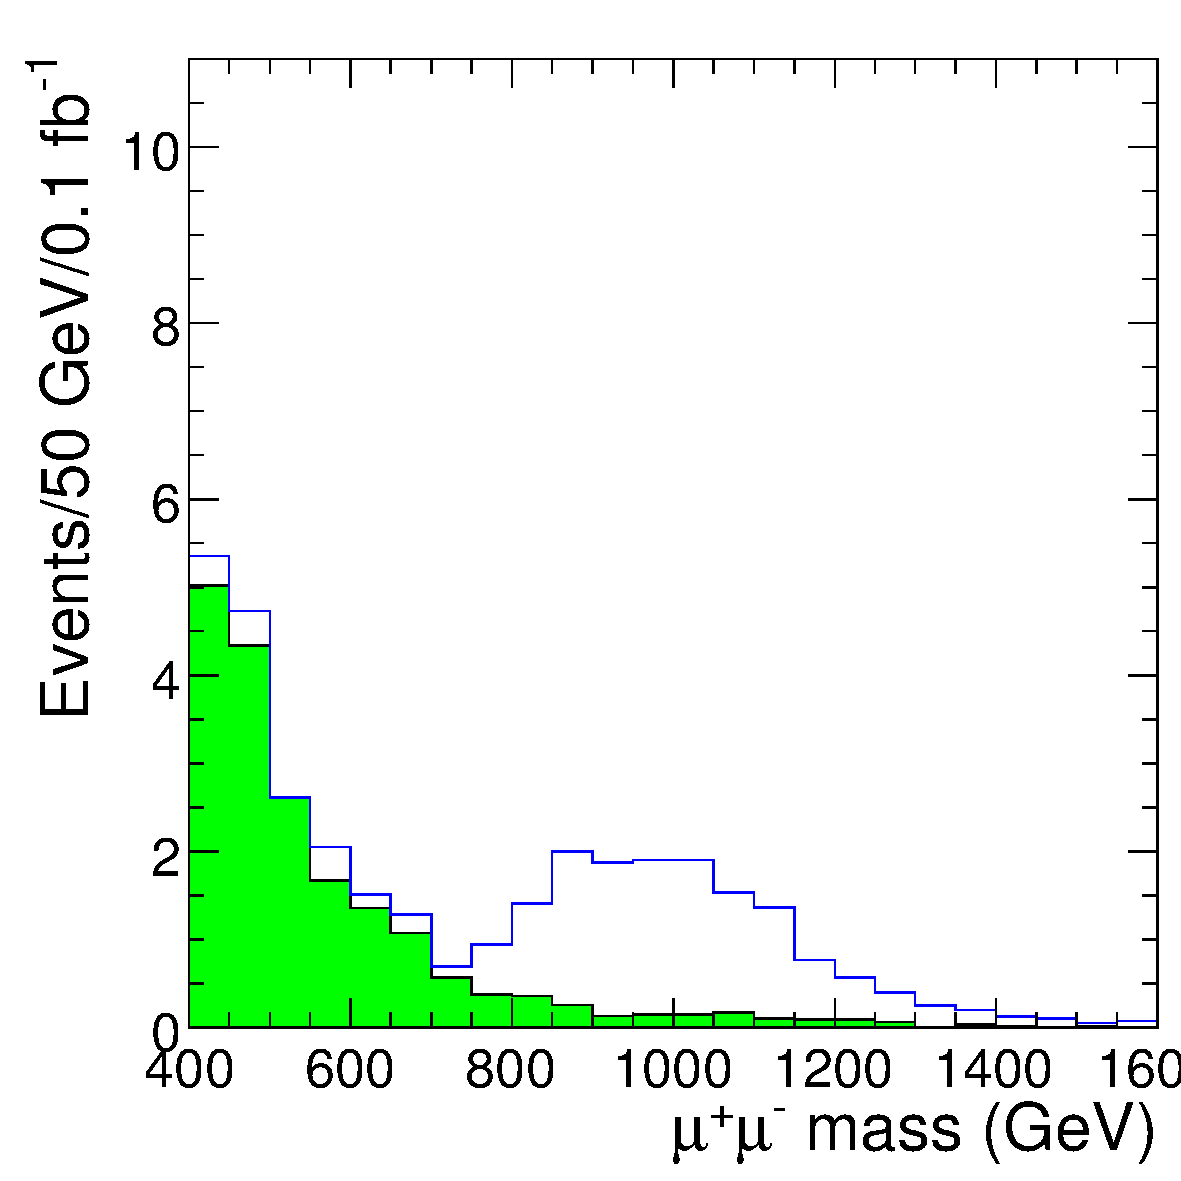
\includegraphics[width=\linewidth]{plots/zmumu/Figure_003-019-b.pdf}
  \end{minipage} &
  \begin{minipage}{\linewidth}
    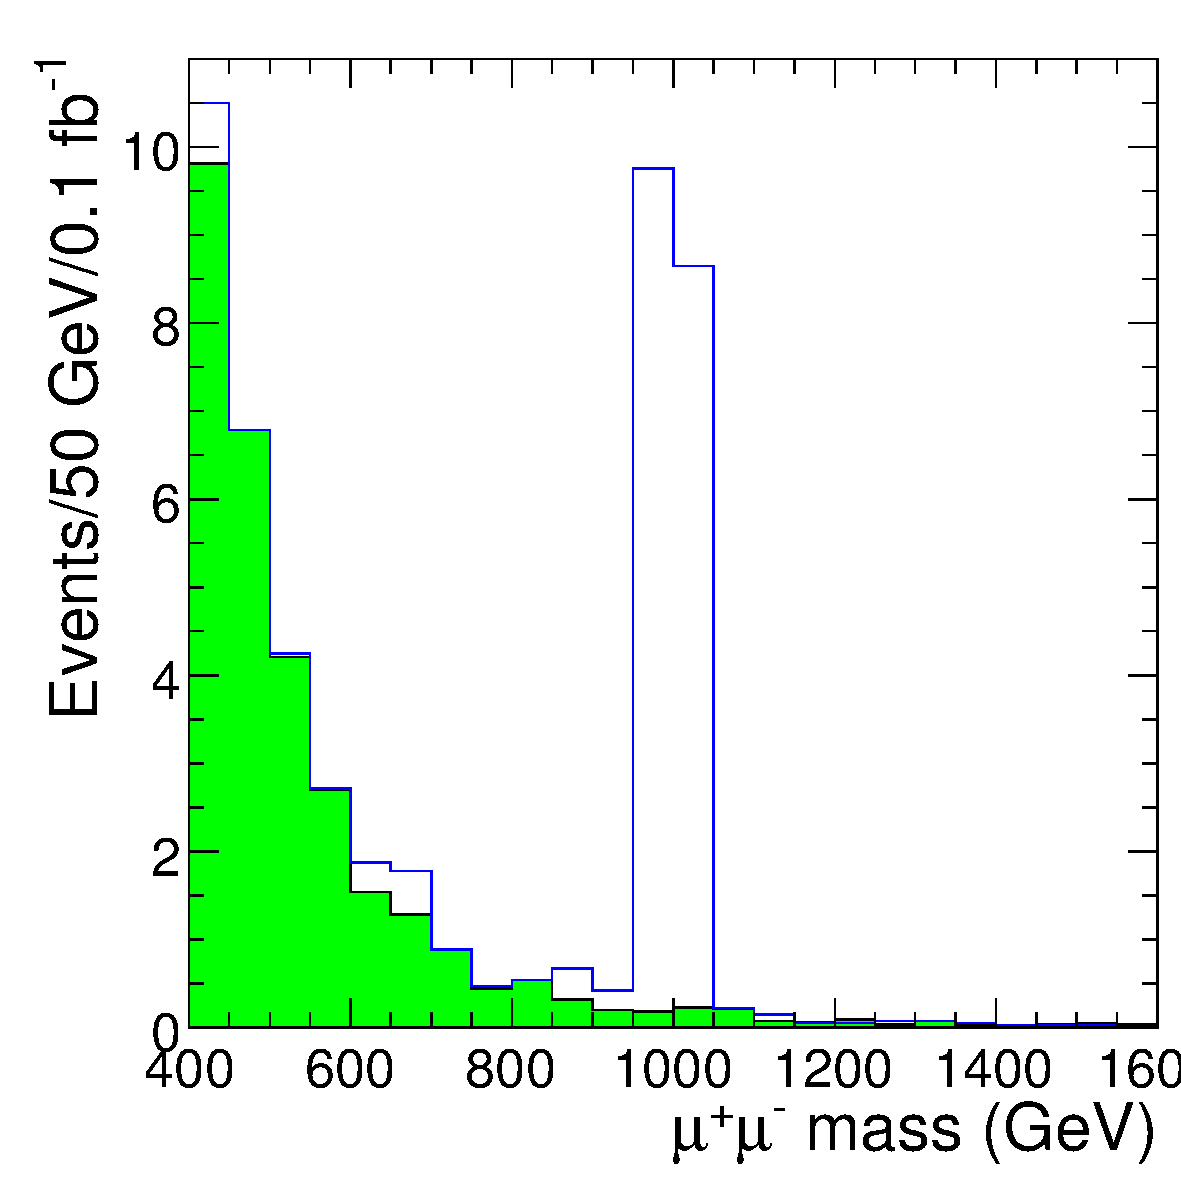
\includegraphics[width=\linewidth]{plots/zmumu/Figure_003-019-a.pdf}
  \end{minipage} \\
  \begin{minipage}{\linewidth}
    \begin{center}
      \mbox{\hspace{0.25 cm}} ``First data'' misalignment
    \end{center}
  \end{minipage} &
  \begin{minipage}{\linewidth}
    \begin{center}
      \mbox{\hspace{0.25 cm}} Ideal alignment
    \end{center}
  \end{minipage}
\end{tabular}
\end{frame}

\begin{frame}
\frametitle{Muon chambers are important for resolution at high $p_T$}
\begin{center}
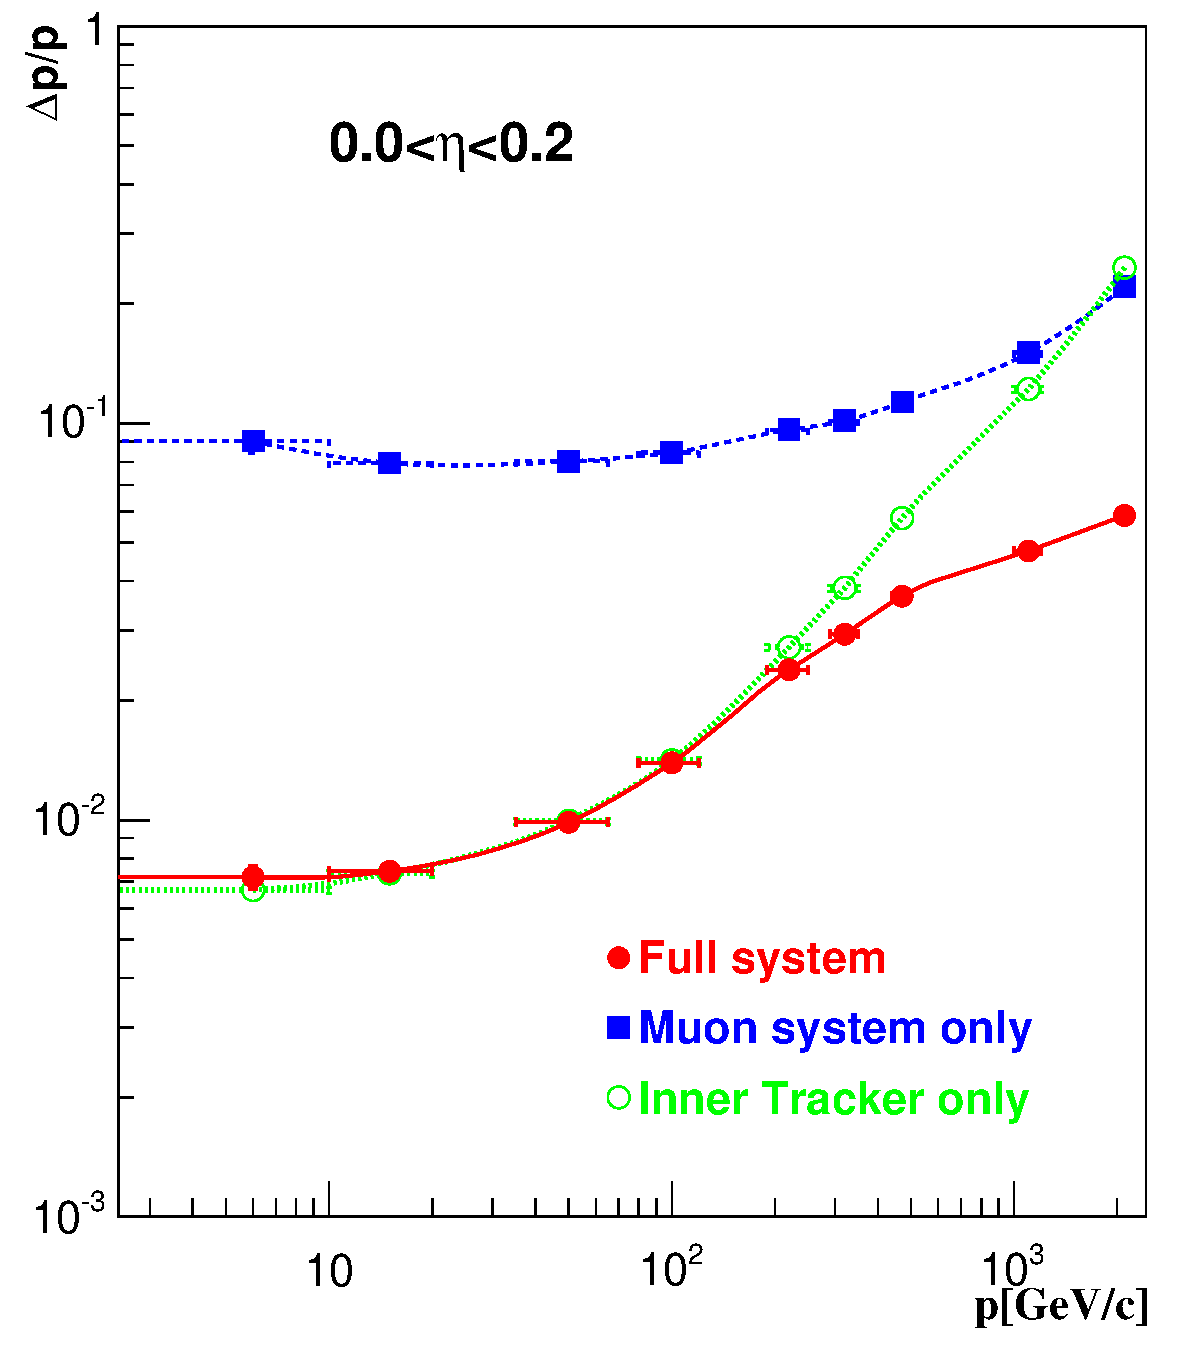
\includegraphics[width=0.45\linewidth]{plots/zmumu/Figure_001-005-a.pdf}
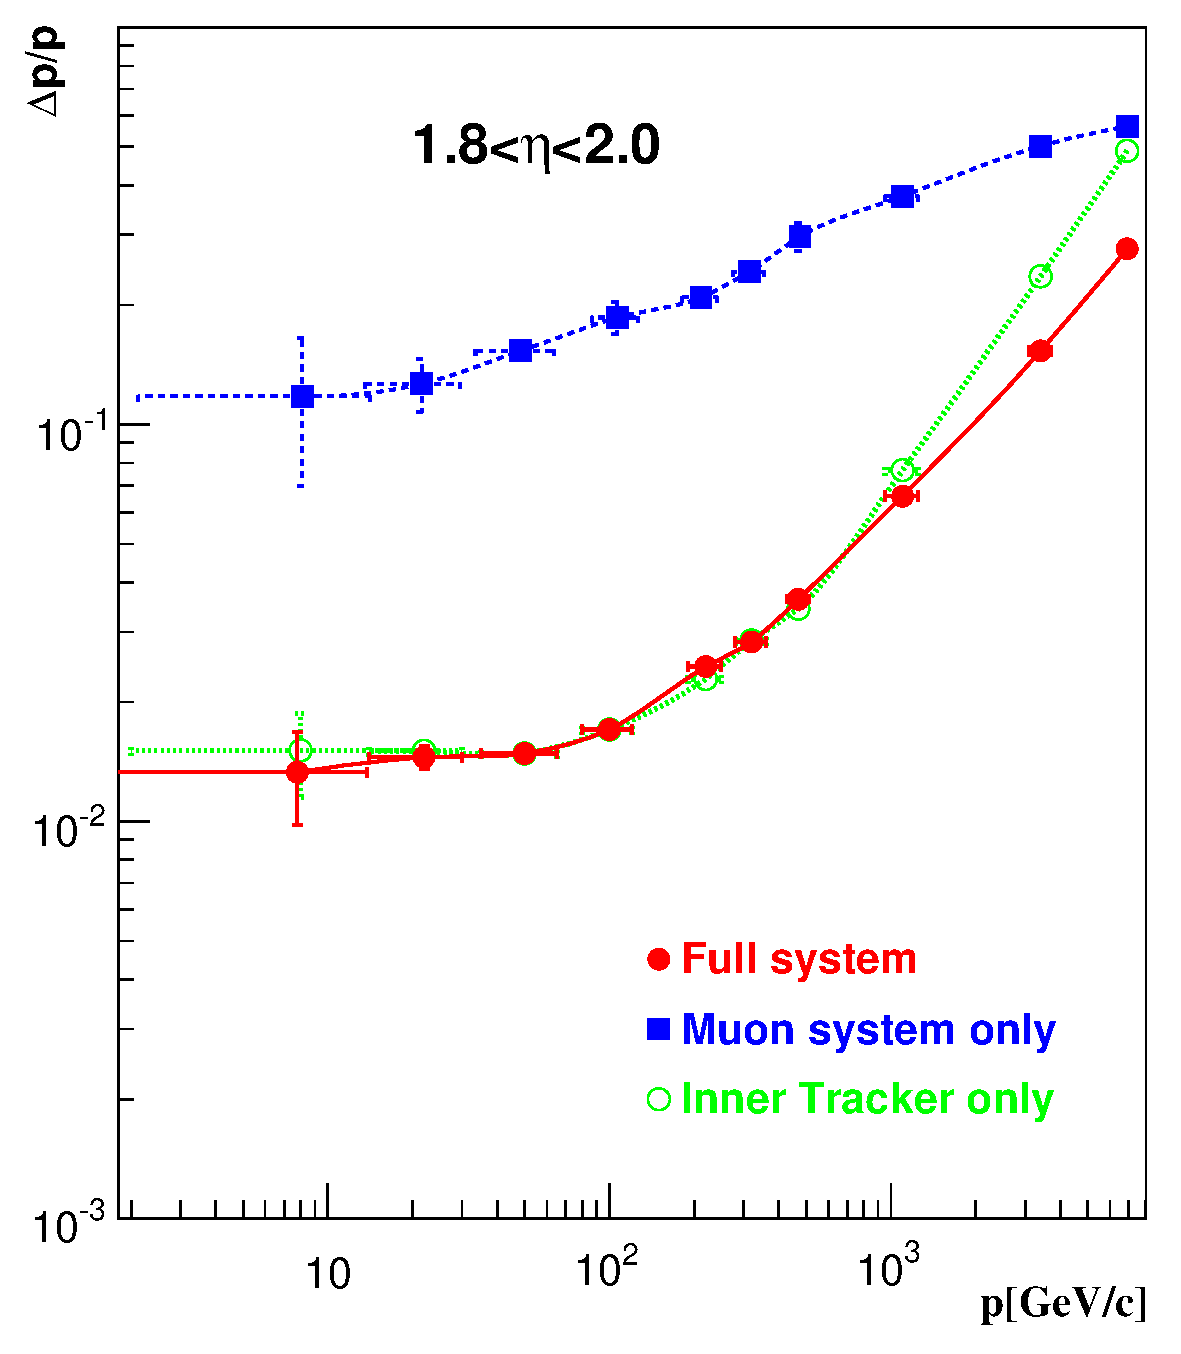
\includegraphics[width=0.45\linewidth]{plots/zmumu/Figure_001-005-b.pdf}
\end{center}

\vspace{-0.5 cm}
\begin{itemize}
  \item Very straight tracks, long lever arm helps!
\end{itemize}
\end{frame}

\section*{Track-based Muon Alignment at CMS --- Jim Pivarski}

\begin{frame}
\frametitle{Muon chamber alignment with tracks}
\begin{itemize}
  \item Provides the final alignment that will be used for $Z'\to\mu\mu$
  \item A\&M's expertise:
  \begin{itemize}
    \item CDF muon reconstruction
    \item Pivarski was CLEO's alignment expert (2000--2004)
  \end{itemize}
  \item<2> Simple, transparent approach: iteratively move chambers to minimize residuals
\end{itemize}

\vspace{-1.1 cm}
\uncover<2>{\begin{center}
\begin{tabular}{p{0.31\linewidth} p{0.31\linewidth} p{0.31\linewidth}}
  \begin{minipage}{\linewidth}
    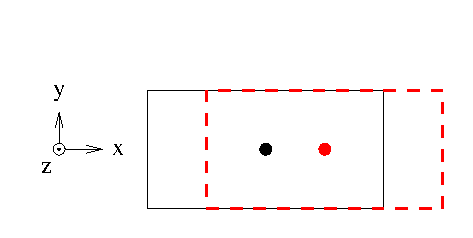
\includegraphics[width=\linewidth]{dof_x}
  \end{minipage} &
  \begin{minipage}{\linewidth}
    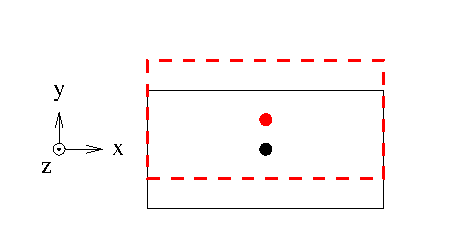
\includegraphics[width=\linewidth]{dof_y}
  \end{minipage} &
  \begin{minipage}{\linewidth}
    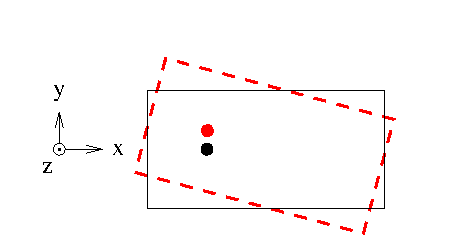
\includegraphics[width=\linewidth]{dof_phiz}
  \end{minipage} \\
  \begin{minipage}{\linewidth}
    \begin{center}
      $x$: offset in $r_x$
    \end{center}
  \end{minipage} &
  \begin{minipage}{\linewidth}
    \begin{center}
      $y$: offset in $r_y$
    \end{center}
  \end{minipage} &
  \begin{minipage}{\linewidth}
    \begin{center}
      $\phi_z$: $r_x$ linear in $y$ and $r_y$ linear in $x$
    \end{center}
  \end{minipage}
\end{tabular}
\end{center}}

\vspace{-0.3 cm}
\uncover<2>{\begin{itemize}
  \item Began CMS muon alignment in October 2006
  \item Combined barrel $+$ endcap alignment
\end{itemize}}
\end{frame}

\begin{frame}
\frametitle{Software development is nearly done}

Integrated our muon alignment code into CommonAlignment
\begin{center}
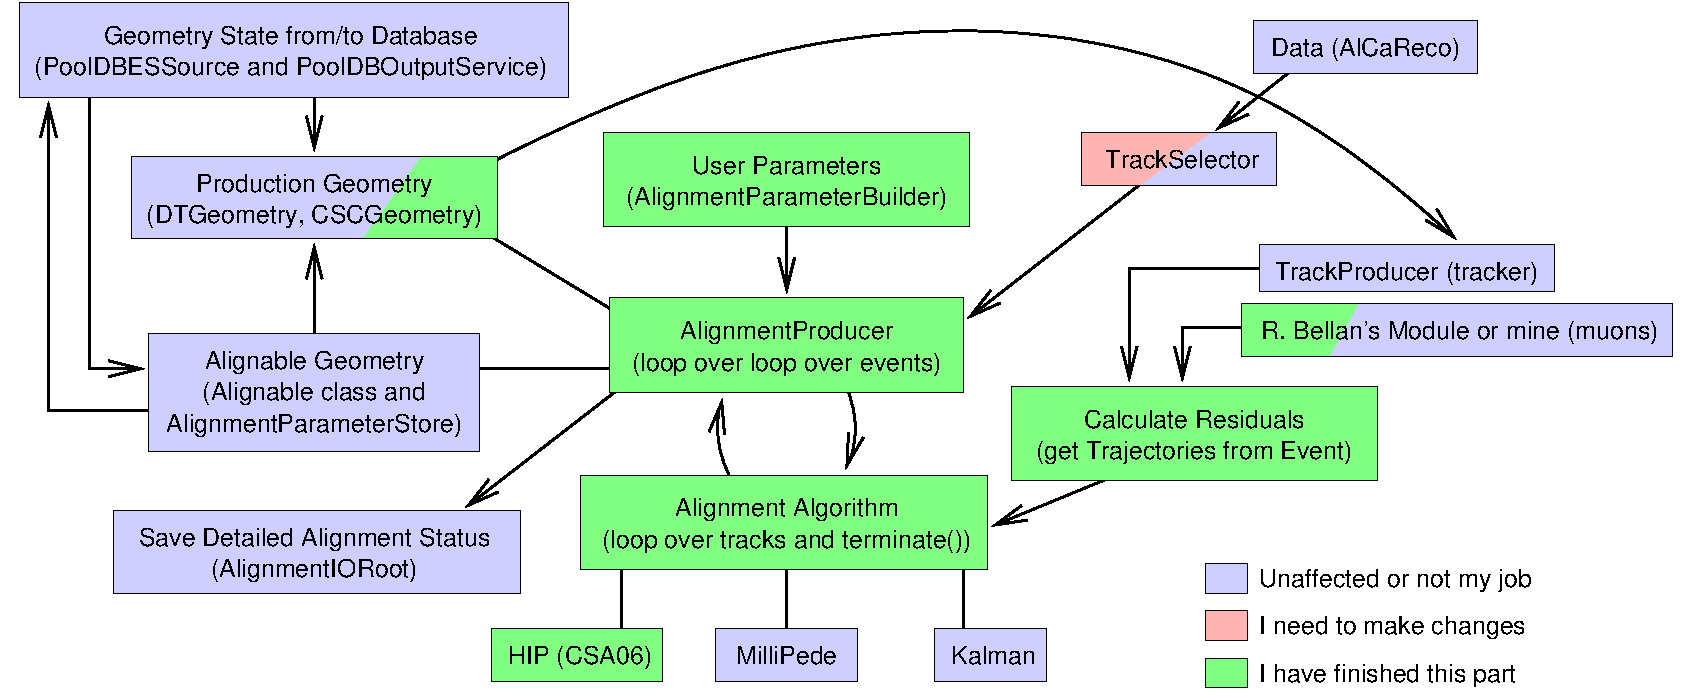
\includegraphics[width=0.9\linewidth]{plots/mine/software_flow_chart}
\end{center}

\begin{itemize}
  \item Unifies tracker alignment and muon chamber alignment
  \item Easy to apply global-fit algorithms to muon chambers
    (MillePede and Kalman-based, in development)
\end{itemize}
\end{frame}

\begin{frame}
\frametitle{Beginning study of alignment procedure}

\begin{tabular}{p{0.3\linewidth} p{0.65\linewidth}}
  \begin{minipage}{\linewidth}
    \vspace{-0.5 cm}
    Potential sources
    \begin{itemize}
      \item $Z\to\mu\mu$
      \item $W\to\mu\nu$
      \item $b\to\mu X$
      \item beam halo, cosmics
    \end{itemize}
  \end{minipage} &
  \begin{minipage}{\linewidth}
    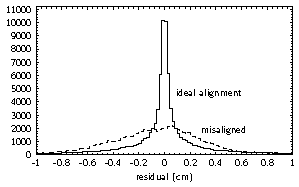
\includegraphics[width=\linewidth]{plots/mine/alignment_residuals.pdf}
  \end{minipage}
\end{tabular}

\vfill
At high luminosity ($10^{33}/$cm$^2/$s, scheduled for 2008), \\ $Z\to\mu\mu$ and $W\to\mu\nu$ will be sufficient:

\vspace{-0.25 cm}
\begin{center}
  17 hours for 200-300 $\mu$m in barrel (410,000 muons), \\ 10 hours for 100-150 $\mu$m in endcap (220,000 muons)
\end{center}
\end{frame}

\section*{Hardware Muon Alignment at CMS --- Jim Pivarski}

\begin{frame}
\frametitle{Hardware EMU alignment system}
Active collaboration with Wisconsin, FIT, FermiLab
\begin{center}
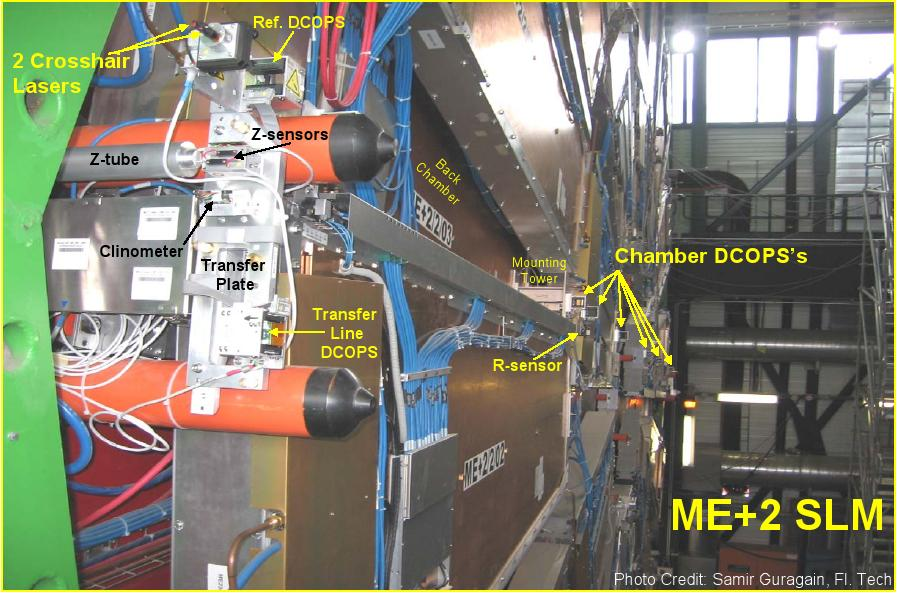
\includegraphics[width=0.8\linewidth]{plots/hw_alignment/photo.jpg}
\end{center}
\end{frame}

\begin{frame}
\frametitle{Contribution to laser alignment}
\begin{tabular}{p{0.6\linewidth} p{0.35\linewidth}}
  \begin{minipage}{\linewidth}
    DCOPS sensor boxes measure position along laser line spanning
    EMU disk

    \vspace{0.25 cm} Existing algorithm computes mean of laser light
    peak\uncover<2->{, sensitive to pathologies:}

  \end{minipage} &
  \begin{minipage}{\linewidth}
    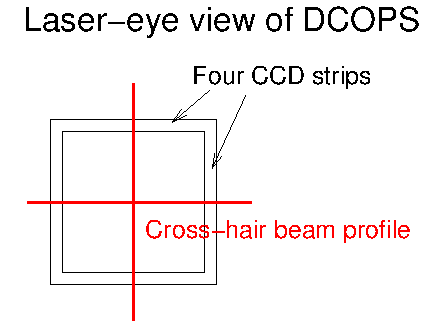
\includegraphics[width=\linewidth]{plots/hw_alignment/laser_crosshairs}
  \end{minipage}
\end{tabular}

\uncover<2->{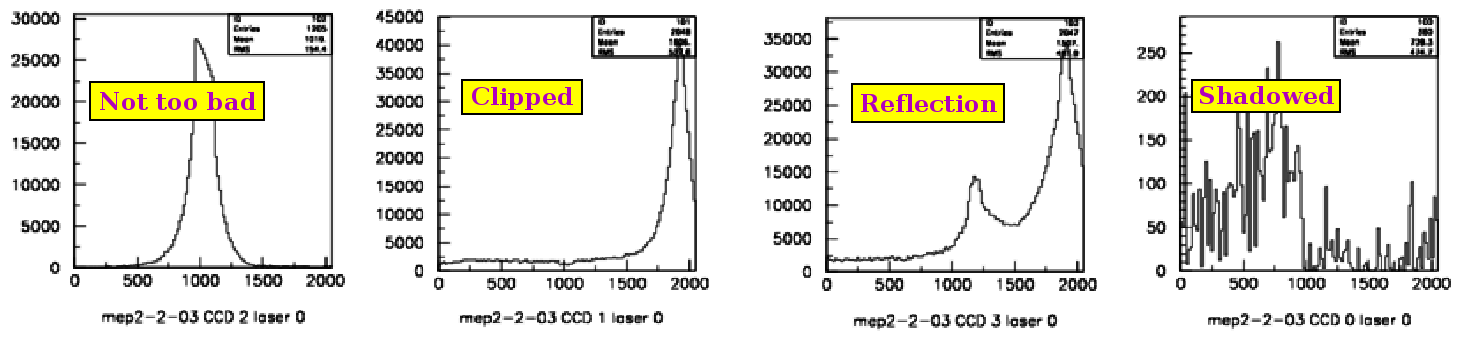
\includegraphics[width=\linewidth]{plots/hw_alignment/bad_dcops.png}}

\uncover<3>{\begin{itemize}
\item Dmitry Yakorev (A\&M grad student) developing algorithms
\item Golyash (our engineer) is reprogramming firmware
\end{itemize}}
\end{frame}

\section*{Super-CMS EMU Upgrade --- Jim Pivarski}

\begin{frame}
\frametitle{Super-CMS EMU upgrade}

\begin{itemize}
  \item c.\ 2015, LHC upgrade to $10^{35}/$cm$^2/$s: a trigger challenge!
  \item<2> Current CMS trigger does not include tracking in Level 1
\end{itemize}

\vspace{-0.5 cm}
\begin{center}
\uncover<2>{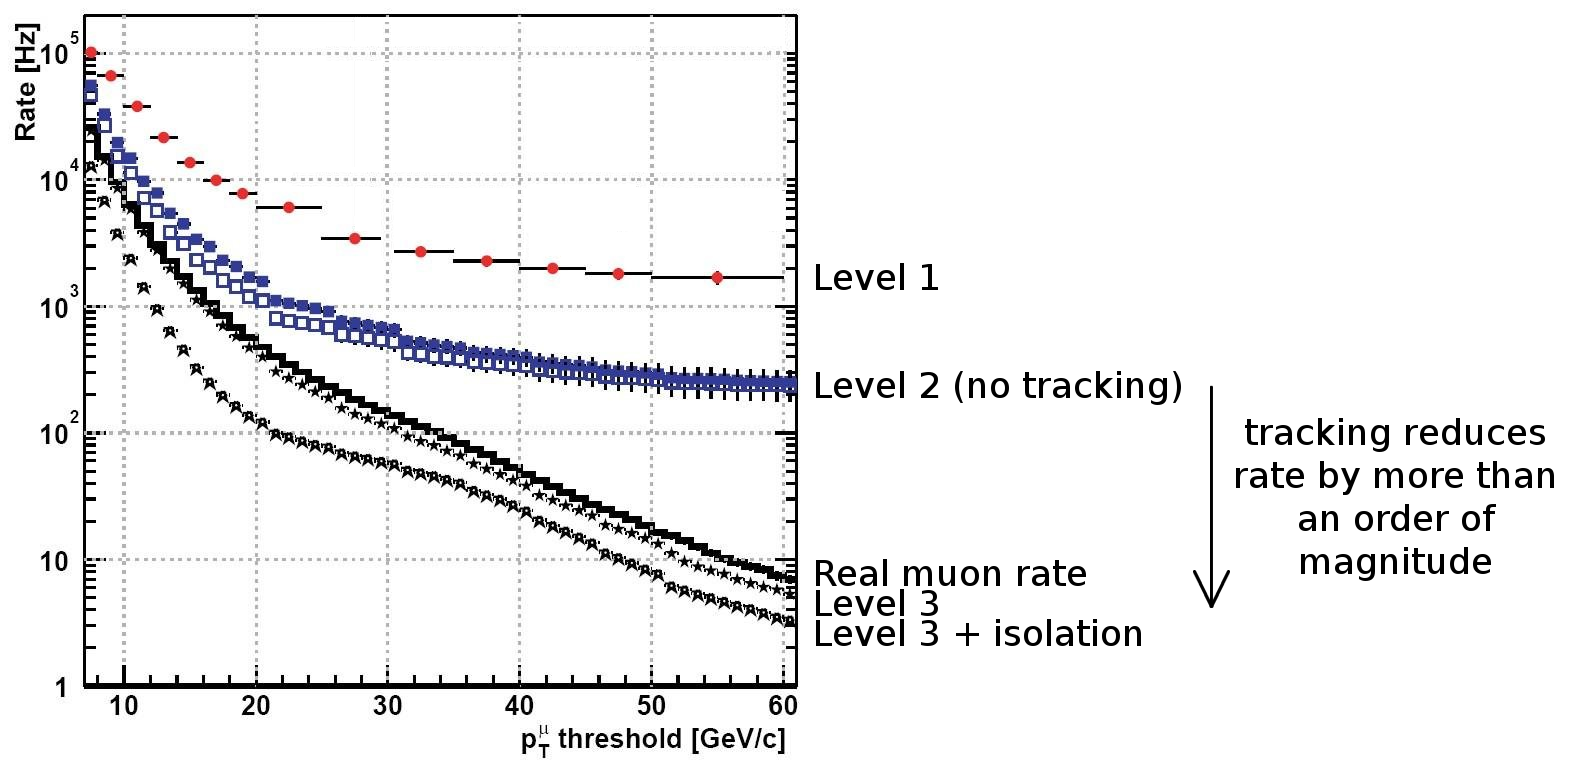
\includegraphics[width=0.8\linewidth]{plots/slhc.png}}
\end{center}

\vspace{-0.5 cm}
\uncover<2>{\begin{itemize}
  \item Plan to work on design of the upgraded trigger system for Super-CMS (Yakorev, Kamon, Safonov)
  \item Both EMU and global trigger
\end{itemize}}
\end{frame}

\begin{frame}
\frametitle{Recap of A\&M muon projects}

{\bf CDF}

\begin{itemize}
  \item Muon reconstruction (Krutelyov, Kamon)
  \item Low-$p_T$ di-muon trigger (Krutelyov, Kamon)
  \item $B_s\to\mu\mu$ analysis (Weinberger, Kamon)
\end{itemize}

{\bf CMS}

\begin{itemize}
  \item EMU low voltage and monitoring (Golyash, Pivarski, Safonov)
  \item $Z'\to\mu\mu$ analysis (Pivarski, Safonov, Kamon)
  \item Track-based alignment (Pivarski, Safonov, Kamon)
  \item Hardware alignment (Golyash, Yakorev, Pivarski, Safonov, \\ \hfill Kamon)
\end{itemize}

\vspace{-\baselineskip}
{\bf Super-CMS}

\begin{itemize}
  \item EMU upgrades (Yakorev, Kamon, Safonov)
\end{itemize}

\label{numpages}
\end{frame}

\end{document}
